\chapter{Experimental Analysis}\label{C11}

Appendix: growing tmax + farsighted vs myopic + framework codice esperimenti

\begin{table}
	\centering
	\begin{tabular}{|c|c|c|c|c|c|c|} 
		\hhline{~------|}
		\multicolumn{1}{l|}{}     & \multicolumn{2}{c|}{{\cellcolor[rgb]{0.878,0.878,0.878}}\textbf{Persistency}}                              & \multicolumn{2}{c|}{\textbf{Tmax}} & \multicolumn{2}{c|}{{\cellcolor[rgb]{0.878,0.878,0.878}}\textbf{Reward}}                                 \\ 
		\hline
		\textbf{Experiment name}  & {\cellcolor[rgb]{0.878,0.878,0.878}}\textit{General} & {\cellcolor[rgb]{0.878,0.878,0.878}}\textit{Thight} & \textit{Known} & \textit{Unknown}  & {\cellcolor[rgb]{0.878,0.878,0.878}}\textit{P.R.} & {\cellcolor[rgb]{0.878,0.878,0.878}}\textit{N.P.R.}  \\ 
		\hline
		\textit{synthetic A}      & {\cellcolor[rgb]{0.878,0.878,0.878}}                 & {\cellcolor[rgb]{0.878,0.878,0.878}}x               & x              &                   & {\cellcolor[rgb]{0.878,0.878,0.878}}x             & {\cellcolor[rgb]{0.878,0.878,0.878}}                 \\ 
		\hline
		\textit{synthetic B}      & {\cellcolor[rgb]{0.878,0.878,0.878}}                 & {\cellcolor[rgb]{0.878,0.878,0.878}}x               & x              &                   & {\cellcolor[rgb]{0.878,0.878,0.878}}x             & {\cellcolor[rgb]{0.878,0.878,0.878}}                 \\ 
		\hline
		\textit{synthetic C}      & {\cellcolor[rgb]{0.878,0.878,0.878}}                 & {\cellcolor[rgb]{0.878,0.878,0.878}}x               &                & x                 & {\cellcolor[rgb]{0.878,0.878,0.878}}x             & {\cellcolor[rgb]{0.878,0.878,0.878}}                 \\ 
		\hline
		\textit{Spotify Scenario} & {\cellcolor[rgb]{0.878,0.878,0.878}}x                & {\cellcolor[rgb]{0.878,0.878,0.878}}                & x              &                   & {\cellcolor[rgb]{0.878,0.878,0.878}}x             & {\cellcolor[rgb]{0.878,0.878,0.878}}                 \\ 
		\hline
		\textit{Rent Scenario}    & {\cellcolor[rgb]{0.878,0.878,0.878}}                 & {\cellcolor[rgb]{0.878,0.878,0.878}}x               & x              &                   & {\cellcolor[rgb]{0.878,0.878,0.878}}              & {\cellcolor[rgb]{0.878,0.878,0.878}}x                \\
		\hline
	\end{tabular}
\caption{Experimental Analysis Summary}
\end{table}
\section{s1}
\begin{figure}[t]
	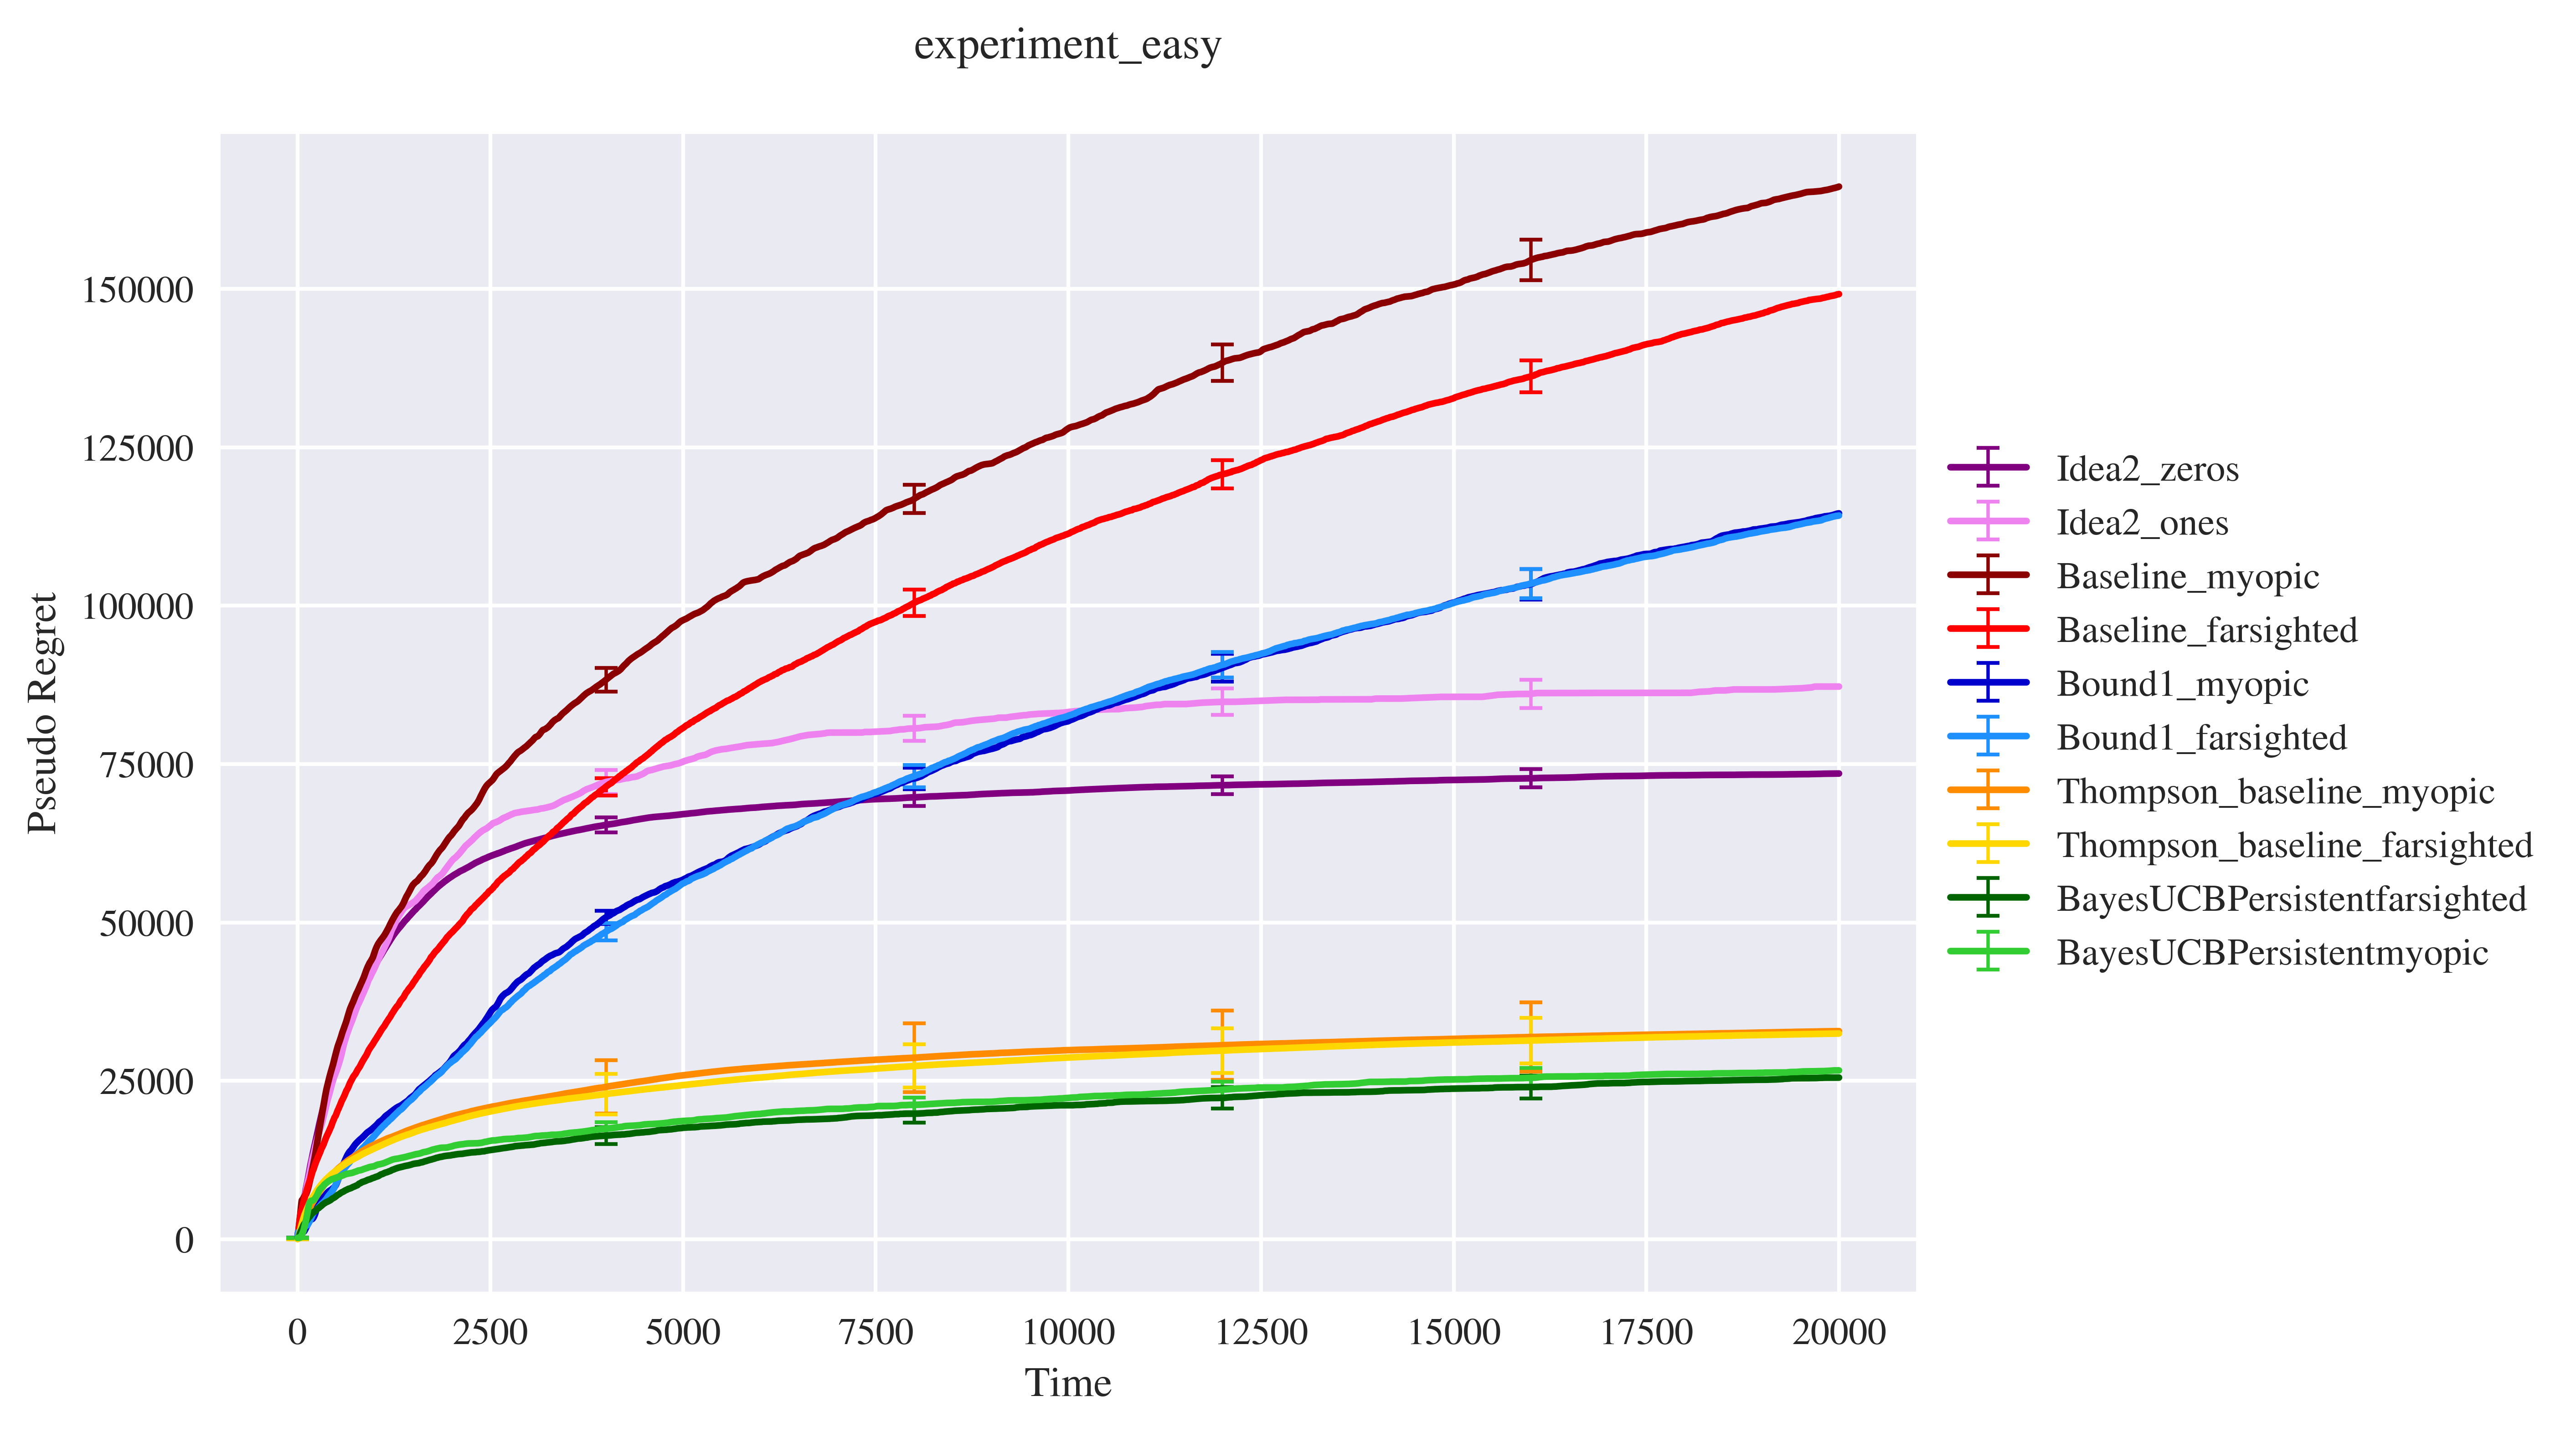
\includegraphics[width=15cm]{./images/experiment_easy ANALYTICS.png}
	\centering	
	\caption{pseudo regret uniformi (R: 1...10) 30 runs Tmax=50}
\end{figure}

